\chapter{TECHNOLOGIES USED}
\section{React-native}
\subsection{About}
React Native is the next generation of React - a JavaScript code library developed by Facebook and Instagram, which was released on Github in 2013. Native app creation simply means writing apps for a specific operating system. React Native helps developers reuse code across the web and on mobile. React Native lets you build mobile apps using only JavaScript. It uses the same design as React, letting you compose a rich mobile UI from declarative components.With React Native, you don’t build a "mobile web app”, an "HTML5S app", or a “hybrid app”. You build a real mobile app that’s indistinguishable from an app built using Objective-C or Java. React Native uses the same fundamen- tal UI building blocks as regular iOS and Android apps. You just put those building blocks together using JavaScript and React.

\subsection{Advantages of React-native}
React Native lets you build your app faster. Instead of recompiling, you can reload your app instantly. With Hot Reloading, you can even run new code while retaining your application state.
React Native combines smoothly with components written in Objective-C, Java, or Swift. It’s simple to drop downto native code if you need to optimize a few aspects of your application. It’s also easy to build part of your app in React Native, and part of your app using native code directly - that’s how the Facebook app works.
The biggest difference is that its cross platform i.e engineers won’t have to build the same app for iOS and for Android from scratch, they can reusing the code across each operating system.

\subsubsection{Still Improving}
React Native isn’t perfect, in fact, it does have some clear limitations.
Some custom modules are missing, meaning that you might lose out on some of its time-saving perks but having to build and create your own.
\vspace{3cm}

\subsubsection{Still technical}
It’s easy to get swept up in React Native’s pre-packaged elements. However, for certain things, you'll still need a developer at hand to take care of some technical nasties.
These include incorporating smartphone camera accessibility into an app or push notifications and more sophisticated data handling.

\subsubsection{Dynamic code updates}
React Native is unique it its ability to push updates to devices without requiring an app release.\\
\begin{figure}[!h]
	\centering
	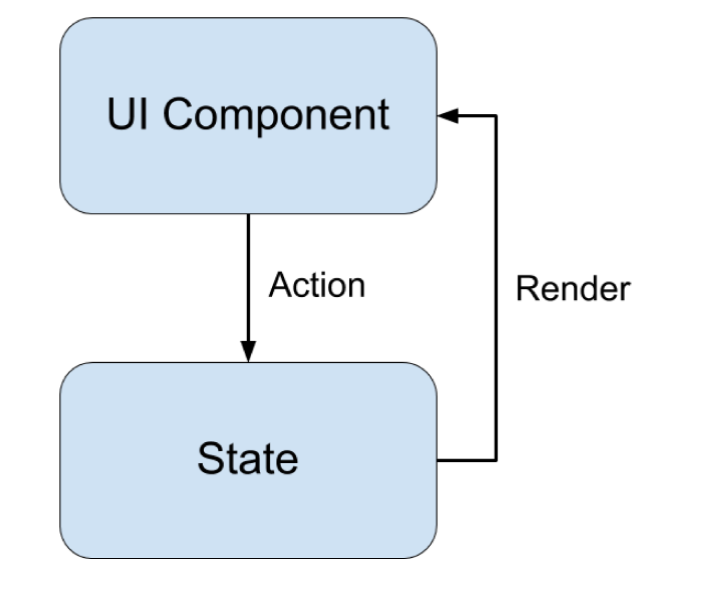
\includegraphics[height=5in]{reactArch.PNG}
	\caption{React Architechture}
	
\end{figure}

\subsubsection{Advantages over android studio}
It is cross-platform unlike android studio and can also be integrated with android studio java files.for those we include it in "node modules" directory in the project drectory.

\section{Android Studio AVD}
An Android Virtual Device (AVD) is a configuration that defines the characteristics of an Android phone, tablet, Wear OS, or Android TV device that you wantto simulate in the Android Emulator. The AVD Manager is an interface you can launch from Android Studio that helps you create and manage AVDs.

An AVD contains a hardware profile, system image, storage area, skin, and other properties.

\begin{figure}[!h]
	\centering
	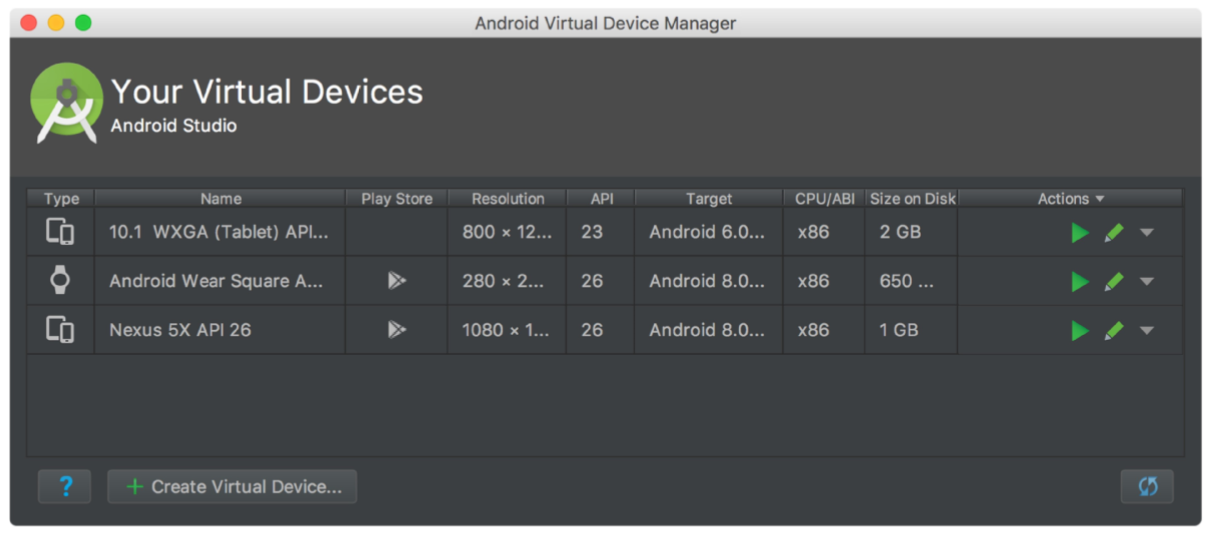
\includegraphics[height=3.1in]{avd.PNG}
	\caption{AVD manager in android studio}
	
\end{figure} 

\subsection{Hardware Profile}
The hardware profile defines the characteristics of a device as shipped from the factory. The AVD Manager comes preloaded with certain hardware profiles, such as Pixel devices, and you can define or customize the hardware profiles as needed.

\subsection{System Image}

We recommend that you create an AVD for each system image that your app could potentially support based on the user sdk setting in your manifest.


\subsection{Storage area}
The AVDhas a dedicated storage area on your development machine. It stores the device userdata, such as installed apps and settings, as well as an emulated SD card. If needed, you can use the AVD Manager to wipe user data, so the device has the same data asif it were new.

\subsection{Skin}
An emulator skin specifies the appearance of a device.Which also include the type of screen ratio your app is capable of supporting the best.


\subsection{Supportability}
AVD is supported only by the processors which support virtualization.

\section{Sublime Text}
Sublime Textis a proprietary cross-platform source code editor with a Python application program- ming interface (API). It natively supports many programming languages and markup languages, and functions can be added byusers with plugins, typically community-built and maintained under free- software licenses.\\
Stable release : 3.0 on 13 September 2017

\section{Firebase}
Firebase provides a realtime database and backend as a service. The service provides application de- velopers an APIthat allows application data to be synchronized across clients and stored on Firebase’s cloud.The company provides client libraries that enable integration with Android, iOS, JavaScript, Java, Objective-C, swift and Node.js applications. The database is also accessible through a REST API and bindings for several JavaScript frameworks such as AngularJS, React, Ember.js and Back- bone.js. The REST API uses the Server-Sent Events protocol, which is an API for creating HTTP connections for receiving push notifications from a server. Developers using the realtime database can secure their data by using the company’s server-side-enforced security rules.[20] Cloud Firestore whichis Firebase’s next generation of the Realtime Database was released for beta use.

\subsection{Properties :}
\subsubsection{Realtime}
Instead of typical HTTP requests, the Firebase Realtime Database uses data synchronization—every time data changes, any connected device receives that update within milliseconds.
\subsubsection{Offline}
Firebase apps remain responsive even when offline because the Firebase Realtime Database SDK persists your data to disk. Once connectivity is reestablished, the client device receives any changes it missed, synchronizing it with the current server state.

\subsection{Working}
The Firebase Realtime Database lets you build rich, collaborative applications by allowing secure access to the database directly from client-side code. Data is persisted locally, and even while offline, realtime events continue to fire, giving the end user a responsive experience. When the device regains connection, the Realtime Database synchronizes the local data changes with the remote updates that occurred while the client was offline, merging any conflicts automatically.
The Realtime Database provides a flexible, expression-based rules language, called Firebase Realtime Database Security Rules, to define how yourdata should be structured and when data can be read from or written to. When integrated with Firebase Authentication, developers can define who has access to what data, and how they can access it.
The Realtime Database is a NoSQL database and as such hasdifferent optimizations and functionality compared to a relational database. The Realtime Database APIis designed to only allow operations that can be executed quickly. This enables you to build a great realtime experience that can serve millions of users without compromising on responsiveness. Because ofthis, it is important to think about how users need to access your data and thenstructure it accordingly.

\subsubsection{Implementation}

1.Integrate the Firebase Realtime Database SDKs\\
Quickly include clients via Gradle, CocoaPods, or a script include.\\
\\
2.Create Realtime Database References\\
Reference your JSON data, such as ”users/user:1234/phoneNumber’” to set data or subscribe to data changes.\\
\\
3.Set Data and Listen for Changes\\
Use these references to write data or subscribe to changes.\\
\\
4.Enable Offline Persistence\\
Allow data to be written to the device’s local disk so it can be available while offline.\\
\\
5.Secure your data\\
Use Firebase Realtime Database Security Rules to secure your data.\\
\\


\newpage